\section{Introduction}

Atom-to-atom mapping assigns corresponding atoms across a reaction. It underlies reaction-center identification, template extraction, and the preparation of endpoint structures for mechanistic calculations. A reaction can admit several plausible correspondences, while many different atom-index assignments are chemically equivalent. An algorithm intended to retain alternatives must therefore resolve two questions: which structural choices deserve separate candidates, and which permutations can be represented together?

Existing approaches use learned correspondence signals or graph-based optimization. RXNMapper derives mappings from attention in a reaction language model~\citep{schwaller2021}; LocalMapper learns from chemist-labeled reactions~\citep{chen2024}; and SLAPMapper combines iterative label refinement with sequential linear assignment~\citep{koda2025}. The Golden benchmark provides a common set of annotated reactions for assessing mapping recovery~\citep{lin2022}. For applications requiring alternatives, recovering the annotation somewhere in a returned family is a different objective from producing one correct top-ranked mapping.

Weighted endpoint graphs introduce a further distinction. A permissive matching tolerance can preserve a fragment despite changes in its bond orders, but the corresponding atom shuffles need not preserve the bond events assigned at a finer threshold. Replacing a compressed family by one representative can therefore hide distinct transformations. Likewise, greedily growing one fragment can prevent a neighboring fragment from reaching an alternative assignment.

GRAFT addresses these issues by combining continuous fragment growth, symmetry compression, and branching over fragment placements and priorities (\Cref{fig:algorithm}). Its final representation groups unordered matched fragment pairs and retains the allowed mapping alternatives within each group. A constraint-based decoder projects these families onto distinct bond-event patterns. The method searches for structurally compatible alternatives without requiring the reference transformation to minimize the number of bond changes.

\section{Method}

\subsection{Weighted matching and continuous growth}

Let $V_R,V_P$ be the reactant and product atom sets, $Z_R,Z_P$ their element labels, and $W_R,W_P$ their symmetric bond-weight matrices. A partial mapping $m:D\subseteq V_R\rightarrow V_P$ is injective and element compatible. On balanced endpoints, a completed mapping is a bijection. Explicit hydrogen atoms participate in the search. Molecular coordinates can accompany the graphs but do not determine the growth decisions.

The active source graph contains edges with weight at least $b$. Starting from a seed atom, GRAFT grows a connected source fragment $F$ while carrying multiple compatible product placements. A frontier queue prioritizes stronger source edges. To add source atom $u$ with product image $v$, a placement must satisfy
\begin{equation}
 Z_R(u)=Z_P(v),\quad v\notin m(F),\quad
 W_P(v,m(r))\geq b,\quad
 |W_R(u,r)-W_P(v,m(r))|\leq\tau_{\mathrm{iso}}
 \label{eq:match}
\end{equation}
for every active, nonrelaxed source edge $(u,r)$ into $F$. All relevant fragment bonds are checked, rather than only the frontier edge that proposed the extension. Source nonedges do not impose negative matching constraints, so additional product bonds remain possible.

An accepted extension enlarges the fragment and filters its compatible placements. Growth continues even if only one placement remains. An unsupported edge is deferred, and other frontier edges can still be explored. When growth reaches an established fragment, ordinary continuation respects its existing assignments. A fragment saturates when no further admissible extension remains; structurally distinct surviving placements then generate separate continuations for the remaining atoms.

This is a greedy search along each trajectory: an accepted extension can remove placements that would support a different fragment boundary. GRAFT broadens coverage through seed orderings, single-edge constraint relaxations, and local changes in fragment priority. A sweep combines the uncut source graph with searches in which one eligible source edge is omitted. Bond-event evaluation always uses the original endpoint matrices.

\begin{figure}[p]
\centering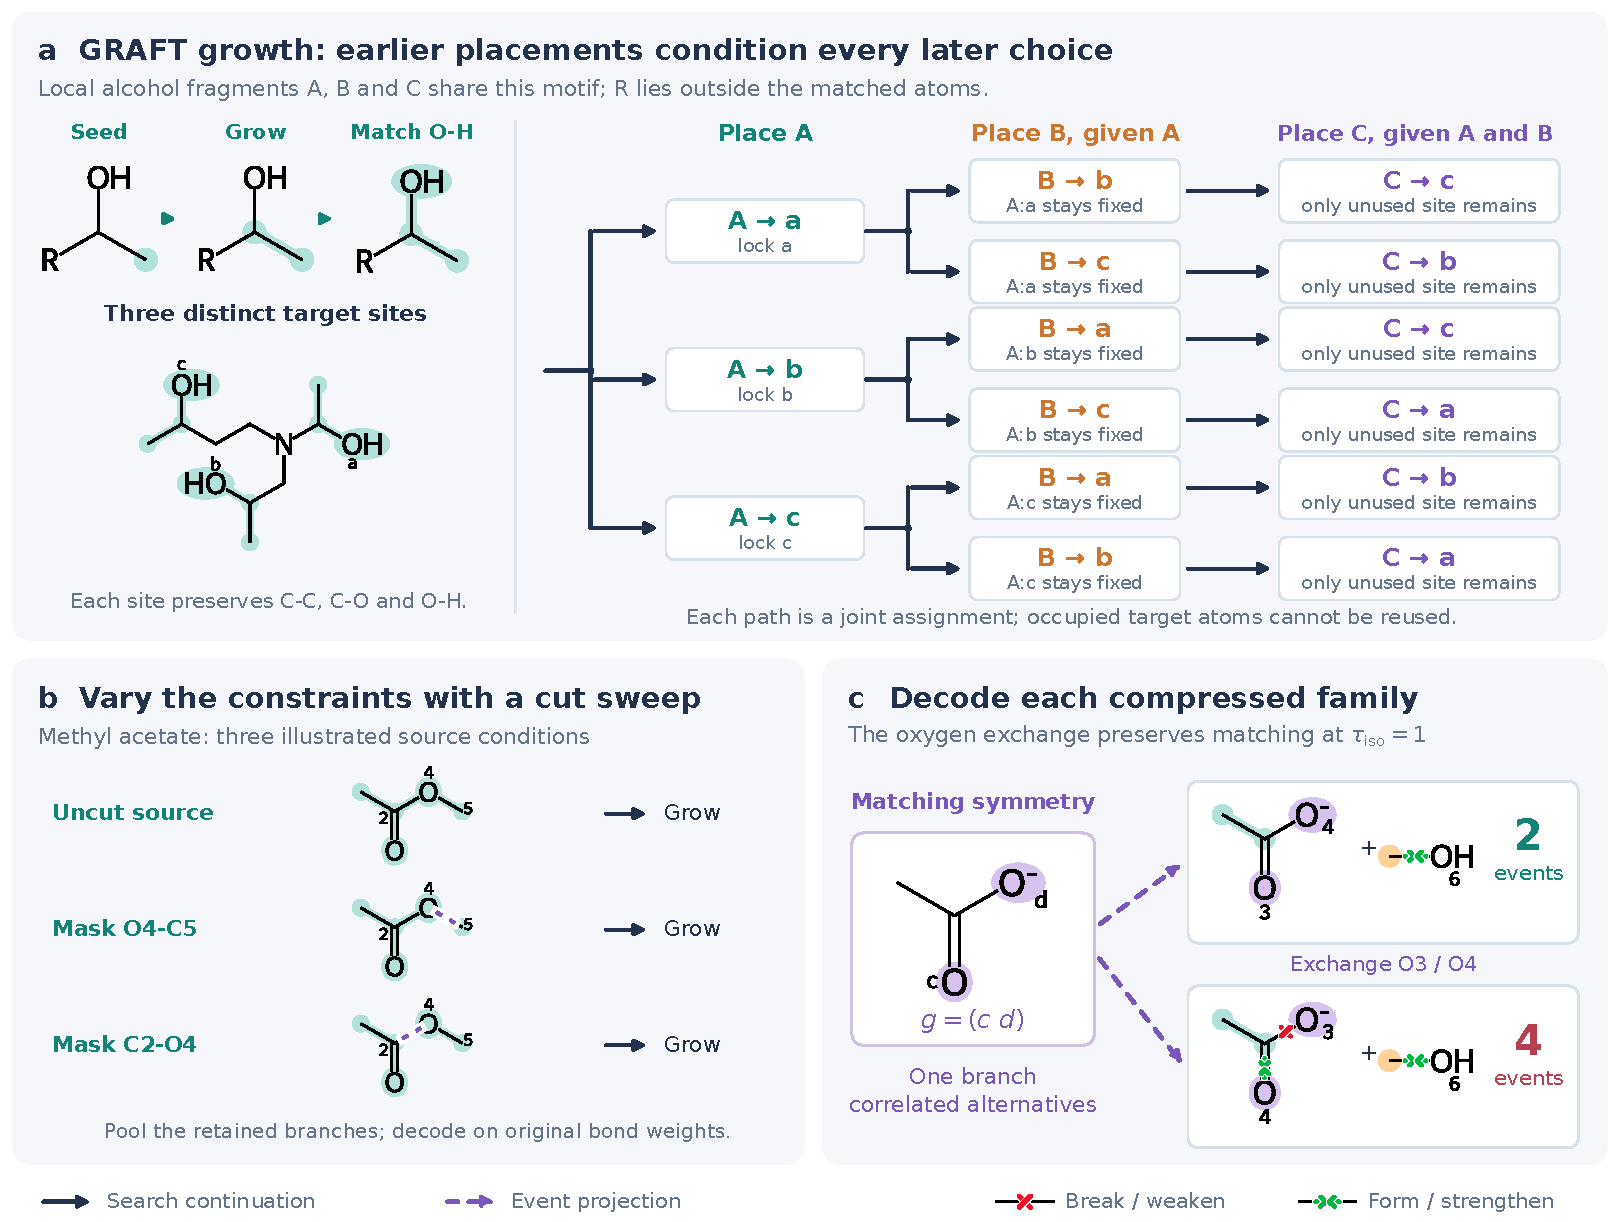
\includegraphics[width=\linewidth]{figs/fig1_algorithm.pdf}
\caption{\textbf{Molecular illustrations of fragment search and event decoding.}
(a) Methyl acetate hydrolysis; reactant indices 1--6 and product indices a--f are independent.
(b) A separate ethanol example shows growth and two admissible images in ethyl lactate; different target atom sets define distinct continuations.
(c) In the hydrolysis fragment, the oxygen exchange $(c\ d)$ preserves matching-response labels at $\tau_{\mathrm{iso}}=1$. Saved constraints govern its admissibility.
(d) Giving B priority transfers O4 from A to B, preserving O4--C5; the original branch remains available.
(e) Oxygen exchange within the original partition changes two heavy-atom events to four at threshold $0.5$.
(f) Those oxygen assignments share an unordered branch but retain different mappings.
These are constructed molecular examples using formal bond orders. Hydrogen transfers are omitted from the illustration; benchmark search and scoring include explicit H.}
\label{fig:algorithm}
\end{figure}

\subsection{Automorphisms and correlated mapping families}

Compatible placements are stored using a representative assignment, unresolved assignment blocks, and permutation generators. During growth, graph canonicalization accounts for the current fragment, locked assignments, and boundary information. Each saved transition records its action generators together with conditioning and fragment-preservation constraints; their conjunction defines the allowed mapping relation. Canonical labeling and automorphism computation use nauty~\citep{mckay2014}.

Matching tolerance and automorphism equivalence have different roles. The relation $|x-y|\leq\tau_{\mathrm{iso}}$ is generally not transitive, so it does not by itself define a permutation group. To describe an intrinsic symmetry shared by a final fragment pair, we instead color product bonds by their responses to the fragment's matching tests. For a product weight $w$ and the set $\mathcal W$ of active reactant weights for the same element pair, the label records
\begin{equation}
 \chi_{\mathcal W}(w)=\left(\mathbf 1[w\geq b],
 \left(\mathbf 1[w\geq b\ \land\ |w-v|\leq\tau_{\mathrm{iso}}]\right)_{v\in\mathcal W}\right).
 \label{eq:response}
\end{equation}
An exact automorphism of this colored graph preserves every encoded matching test. This definition depends on the final fragment pair, not its growth order.

The saved mapping relation also contains the constraints imposed by its search decisions. We represent a flat family $\mathcal F_j$ by a seed mapping $m_j$, a sequence of allowed action groups $G_{j,1},\ldots,G_{j,k}$, and final preservation constraints $C_j$:
\begin{equation}
 \mathcal F_j=\left\{a_k\circ\cdots\circ a_1\circ m_j:
 a_i\in G_{j,i},\ C_j(a_k\circ\cdots\circ a_1\circ m_j)\right\}.
 \label{eq:family}
\end{equation}
These actions encode correlated moves; atoms in a common orbit are not independently permutable. Disjoint actions commute and can be placed in a canonical order. The order of overlapping actions is retained. A sequence of groups is not generally equivalent to the group generated by their union.

The intrinsic automorphism of a fragment pair is shared metadata, not permission to enlarge its saved family. Multiple admissible seed mappings can occupy different intrinsic symmetry orbits, and different search constraints can restrict the allowed actions. GRAFT therefore retains these alternatives explicitly inside the compressed representation.

\subsection{Branching through fragment competition}

Saturated-placement branching explores different images of a fragment. Fragment competition additionally explores a different division of the source atoms. Suppose established fragment $A$ borders fragment $B$. In a challenger branch, GRAFT rematches $B$ together with a contacting atom of $A$, allowing the challenger to occupy a different compatible product region. Assignments conflicting with the new placement are released. Unaffected assignments remain anchored, and the fragment-growth procedure fills the resulting gaps. Small attached components can also be released when their assignments depend on the displaced region.

The repaired continuation begins from the revised assignments and constraints; it does not inherit displaced assignments as immutable conditions. Before admission, its complete representatives are checked for element compatibility, injectivity, and preservation of their required fragment bonds. Accepted continuations join the original output, so competition supplements the available alternatives. A finite queue, a bound on successive priority changes, and a completion budget control its cost. Repeated proposals and equivalent completion requests are cached.

\subsection{Unordered final branches}

During search, history and boundary conditions matter because they determine valid continuation. At completion, the branch identity is instead the unordered collection of matched atom sets,
\begin{equation}
 \mathcal B=\{(R_1,P_1),\ldots,(R_q,P_q)\},
 \qquad P_i=m(R_i),
 \label{eq:branch}
\end{equation}
under a fixed matching policy. Sorting atoms within each set and then sorting the fragment pairs removes dependence on growth order and fragment labels. Growing $A$ before $B$ or $B$ before $A$ yields one branch when the final paired sets agree.

Each branch stores the union of its flat families. Identical normalized family records are shared, while distinct constraints or action programs remain available. This transformation preserves the represented mapping union: it changes its grouping, not its admissible assignments. Provenance links retain the discovering paths, but the original search hierarchy is unnecessary for decoding. This conservative deduplication does not assert that the remaining families are mutually disjoint.

\subsection{Decoding distinct bond-event patterns}

For each complete mapping, define the signed change for an unordered source pair $\{u,v\}$ by
\begin{equation}
 \Delta_{uv}(m)=W_P(m(u),m(v))-W_R(u,v),\qquad
 s_{uv}(m)=
 \begin{cases}
 +1,&\Delta_{uv}(m)\geq\delta_{uv},\\
 -1,&\Delta_{uv}(m)\leq-\delta_{uv},\\
 0,&\text{otherwise}.
 \end{cases}
 \label{eq:events}
\end{equation}
Positive events denote bond formation or strengthening; negative events denote cleavage or weakening. The event count is $E(m)=\sum_{u<v}\mathbf 1[s_{uv}(m)\ne0]$. The evaluation includes hydrogen atoms and all atom pairs. For the WBO collection, $\delta_{uv}=0.3$ for pairs involving a metal and $0.5$ otherwise. These thresholds are independent of $\tau_{\mathrm{iso}}$.

The decoder returns one mapping witness per distinct signed event class, identifying patterns related by exact source permutations that preserve the event-response labels. First, symmetry-invariance certificates identify families whose mappings all produce equivalent events, and reachable-image bounds exclude families outside a requested event window. Before constraint encoding, adjacent nested action groups are absorbed: if $H\leq G$, then $HG=GH=G$. Exact generator-membership tests remove these redundant choices without changing the final preservation constraints. Remaining families are encoded symbolically in Z3~\citep{demoura2008}. Each satisfying assignment yields a concrete mapping and its event pattern. A constraint then excludes that entire event-equivalence class, and the process repeats. This projects directly onto event classes rather than explicitly enumerating full mappings or permutation groups.

For a window $E\leq K$, decoding is complete when every retained family is certified exhausted or excluded. A timeout leaves completeness unresolved. This certificate concerns the saved search output within the window; it does not establish exhaustive exploration of all chemically possible mappings. The default deduplication preserves families that contain different event counts, as illustrated in the heavy-atom projection in \Cref{fig:algorithm}e.

\FloatBarrier
\section{Evaluation}

\subsection{Datasets and configurations}

We evaluate annotated mapping recovery on all 1,851 Golden records~\citep{lin2022} and event alternatives on 140 native coordinate/WBO endpoint pairs. Golden inputs use formal bond orders and explicit-H expansion. Reference labels are removed before search. Correctness compares the annotated heavy-atom correspondence, including unmatched atoms, modulo endpoint chemical automorphisms preserving charge, isotope, hydrogen count, and stereochemistry. A recovery requires a verified reference witness among the returned alternatives. Unresolved cases remain in the denominator.

The coordinate collection contains balanced endpoint pairs with 18--137 explicit atoms, including organometallic and multicomponent structures. It has no annotated mappings and was inspected during method development. Its evaluation measures coverage of comparator event classes, not chemical accuracy. SLAP outputs are rescored on the same original WBO matrices using \Cref{eq:events}. Each returned heavy-atom assignment is completed by symbolic hydrogen refinement. The comparator classes are those observed among these returned witnesses; its hydrogen label families are not exhaustively decoded.

\begin{table}[tb]
\centering\small
\caption{\textbf{Evaluation configurations.} Both use $b=0.2$, $\tau_{\mathrm{iso}}=1$, explicit H, and uncut plus single-edge searches. A seed setting counts source-atom orderings per cut.}
\label{tab:protocol}
\begin{tabular}{lcc}\toprule
Setting & Golden & Coordinate/WBO\\\midrule
Reactions & 1,851 & 140\\
Search directions & Both, unioned & Reactant to product\\
Seed orderings & 1, 2, 3, 10 & 1\\
Branch cap & 100 & 2,000\\
Competition completions per reaction & 0 & Up to 128\\
Evaluation & Reference-family recovery & Signed event-class coverage\\\bottomrule
\end{tabular}
\end{table}

\Cref{tab:protocol} separates the settings actually evaluated. Golden measures the fragment-search stage; the 140-case evaluation also includes local competition and final event decoding. The competition configuration considers up to eight distinct parent partitions and two successive priority changes. Its budget was selected on development cases before the full 140-case evaluation. Comparator mappings are not used to propose or accept search branches. A two-order run of the final coordinate pipeline was not performed. Detailed protocols and artifact identifiers are given in \Cref{sec:reproducibility}.

\subsection{Golden mapping recovery}

With one ordering per cut, bidirectional GRAFT recovers \GoldenOneRecovered/1,851 annotated mappings (\GoldenOnePercent\%). Three orderings recover \GoldenThreeRecovered{} (\GoldenThreePercent\%; \Cref{tab:seeds}), and ten recover \GoldenTenRecovered{} (\GoldenTenPercent\%), with \GoldenTenUnknown{} reactions unresolved. Two orderings also recover \GoldenOneRecovered{} (\GoldenOnePercent\%), with no unresolved reactions at either setting. These are family-recovery measurements: they quantify whether a reference correspondence is retained, rather than whether it is ranked first.


\begin{table}[tb]
\centering\small
\caption{\textbf{Golden reference-family recovery and CPU cost.} Recovery uses all 1,851 records. CPU averages use the same \CommonCases{} completed reactions on the Mac, including both directions and the respective sweeps; reference verification is excluded. Dashes mark mixed-host configurations whose times are not compared. ``Absent'' means excluded from saved families; ``unknown'' denotes unresolved verification.}
\label{tab:seeds}
\begin{tabular}{lrrrrr}\toprule
Configuration & Recovered & \% & Absent & Unknown & CPU s/reaction\\\midrule
1 seed order & 1,834 & 99.08 & 17 & 0 & 2.52 \\
2 seed orders & 1,834 & 99.08 & 17 & 0 & 4.95 \\
3 seed orders & 1,837 & 99.24 & 14 & 0 & -- \\
10 seed orders & 1,840 & 99.41 & 9 & 2 & -- \\
SLAP sweep & 1,796 & 97.03 & 52 & 3 & 4.82 \\
\bottomrule\end{tabular}

\end{table}

The SLAP single-edge sweep recovers \SlapRecovered/1,851 references (\SlapPercent\%) using both directions and binary and weighted modes. One-order GRAFT has a higher verified recovery rate by \RecoveryDifference{} percentage points. The paired comparison contains \AamOnly{} references verified only by one-order GRAFT and \SlapOnly{} verified only by SLAP. This compares recovery among alternatives under the stated configurations; it is not a comparison of single-answer accuracy or equal-size candidate sets.

On the same-Mac subset of \CommonCases{} reactions with completed one- and two-order searches and complete SLAP output, mean recorded CPU time is \OneCPU{} seconds per reaction for one-order GRAFT, \TwoCPU{} for two orders, and \SlapCPU{} for the SLAP sweep (\Cref{fig:golden}). Both directions and the respective sweeps are included; reference verification is excluded. GRAFT search-call timing includes checkpoint I/O, whereas SLAP's graph-construction, mapping, and export timers exclude I/O. These are workflow measurements with different output representations. Three- and ten-order searches span Mac and Linux hosts, so their timings are not pooled into a speedup comparison.

\begin{figure}[tb]
\centering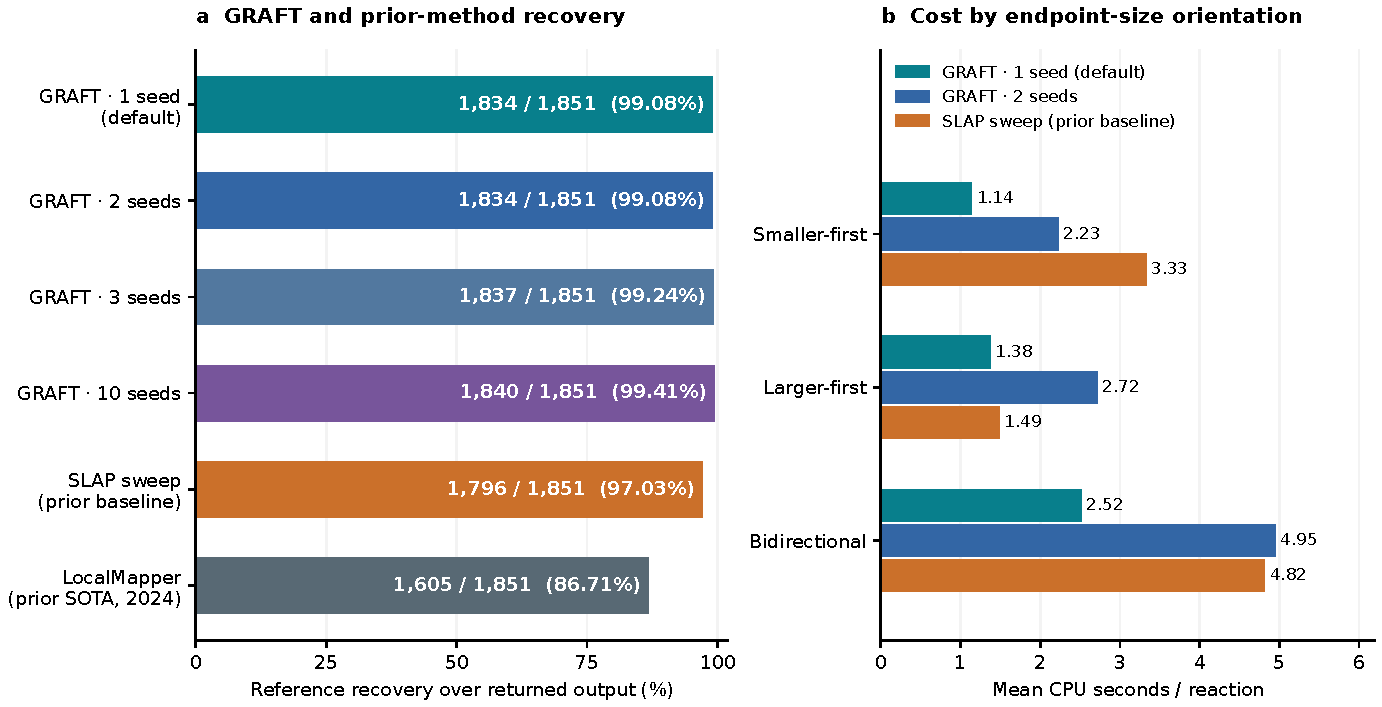
\includegraphics[width=\linewidth]{figs/fig2_golden.pdf}
\caption{\textbf{Reference recovery and search cost.} (a) Golden family recovery for each GRAFT seed setting and the SLAP sweep. Every percentage uses all 1,851 records. (b) Mean recorded workflow CPU on the same \CommonCases{} completed reactions on the Mac. Reference verification is excluded; the procedures have different search objectives, output cardinalities, and I/O timing scopes.}
\label{fig:golden}
\end{figure}

\subsection{Bond-event alternatives on coordinate inputs}

The configuration with fragment competition returns full explicit-atom mappings for all 140 coordinate pairs. Across the collection, it recovers \SweepRecovered{} of the \SweepClasses{} minimum-event classes among the returned SLAP-sweep witnesses, covering every compared class in 139 reactions (\Cref{fig:coordinate}). In the remaining carbocation reaction, it recovers three of five comparator classes. Both searches reach four events there; the difference concerns two alternative patterns at that minimum. Against native SLAP, coverage is 155/160 minimum-event classes, again with all missing classes confined to the same reaction.

Local competition expands the retained event-class set by \CompetitionClasses{} classes across \CompetitionCases{} reactions within the evaluated windows. One added event class in one reaction requires decoding internal family shuffles and is absent from the repair representatives. This demonstrates why final candidate extraction must retain correlated alternatives rather than score only one witness. All accepted competition families were completely decoded within their corresponding event windows; this does not imply that every search trajectory was explored.

\subsection{Final representation and postprocessing cost}

Unordered fragment-pair deduplication reduces the 140-case total from 237,645 ordered branch records to 124,641 final branches, a 47.55\% reduction. The median falls from 596.5 to 397 branches per reaction. The largest individual reduction is from 52,669 to 2,856 (\Cref{fig:coordinate}).

The final representation retains 236,653 distinct normalized mapping-family records. Thus, fewer branch identities do not imply an equal reduction in event-decoding work: several constrained families can belong to the same fragment combination. Catalogue construction, shared intrinsic symmetry computation, representative checks, and complete event-window decoding together take \DecodeWallMinutes{} minutes of wall time and \DecodeCPUMinutes{} recorded CPU-minutes on three local workers. Peak combined sampled memory is \DecodeGiB{} GiB. These measurements include certificate journaling and bounded continuation, and exclude matching and competition. Other benchmark jobs shared the computer, so the wall time is an observed campaign duration rather than an isolated latency measurement.

Every family in all 140 catalogues was freshly decoded or certified within its specified event window (\Cref{sec:reproducibility}). The output contains \DecodedClasses{} distinct reaction-specific event classes, each with a mapping witness. No case remains unresolved within those windows. Preservation of the family union follows from the transformation in \Cref{eq:family,eq:branch}.

\begin{figure}[tb]
\centering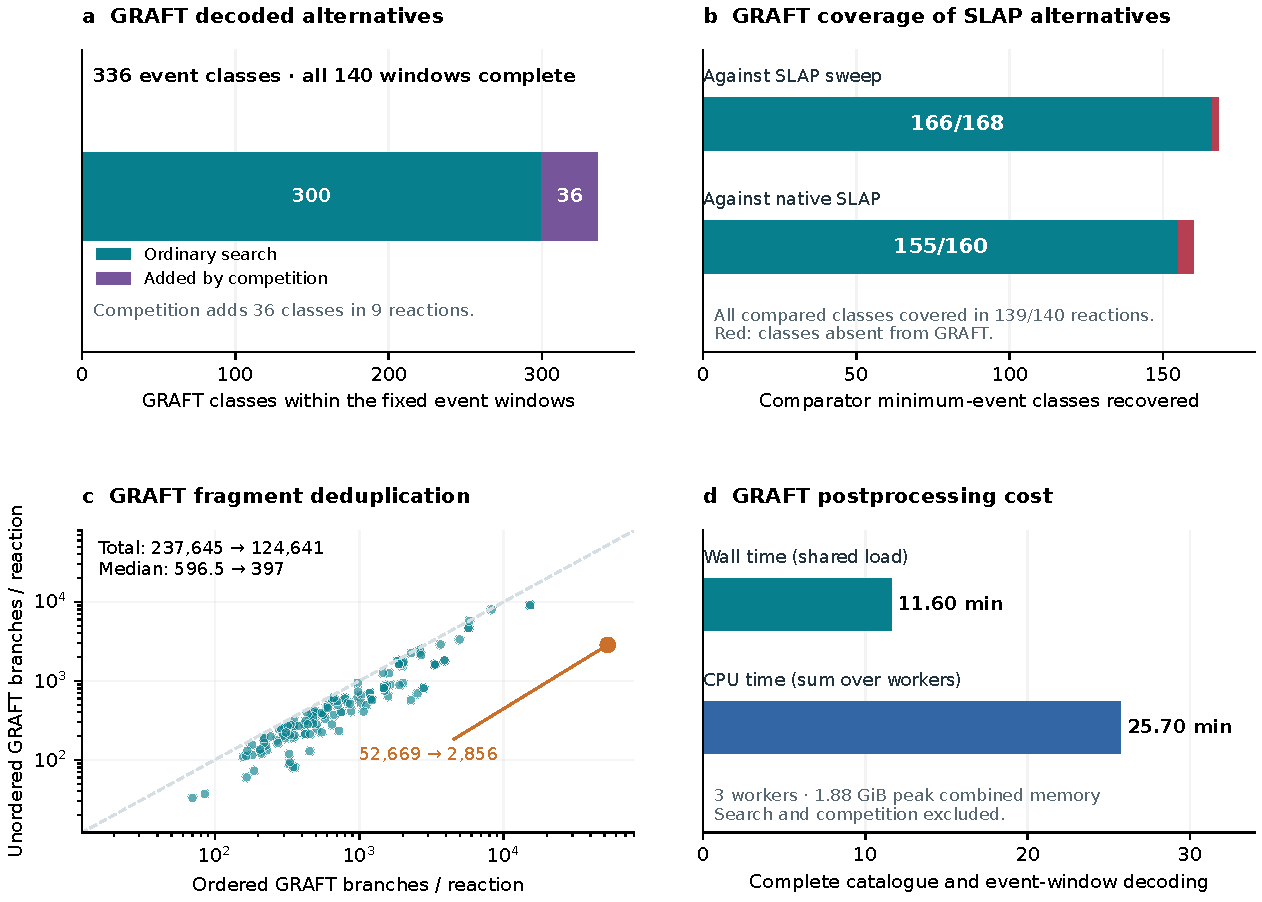
\includegraphics[width=\linewidth]{figs/fig3_coordinate.pdf}
\caption{\textbf{Event alternatives and final branch representation on 140 reactions.}
(a) Recovery of minimum-event classes among fresh comparator witnesses. GRAFT covers every SLAP-sweep class in 139 reactions; the remaining reaction has two missing alternatives at the same four-event minimum.
(b) Per-reaction ordered and unordered branch counts; the diagonal denotes equality. The highlighted case falls from 52,669 to 2,856. Branches are fragment-pair combinations, not counts of explicit mappings or event classes.}
\label{fig:coordinate}
\end{figure}

\FloatBarrier
\section{Discussion}

GRAFT separates structural search, symmetry representation, and interpretation of bond changes. Continuous growth accumulates context while preserving multiple placements; local competition allows neighboring fragments to challenge an established partition. Final grouping removes irrelevant growth order, while the flat family representation retains constraints and correlated permutations that can affect the output. Symbolic projection then exposes distinct bond-event hypotheses without expanding every mapping.

The Golden results support broad reference coverage by the fragment-search stage, and the coordinate results show that the competition configuration retains nearly all minimum-event alternatives found by the SLAP sweep. These are complementary measurements. The coordinate collection has no mapping annotations, and event minimization is not an energy model or a proof of mechanistic plausibility. The priority budget was tuned on development cases, so independent validation is needed to establish generalization.

Finite schedules, greedy growth, branch caps, and competition budgets limit coverage. A complete event-window certificate applies only to the saved families. Matching-preserving automorphisms can change finer-threshold events. GRAFT therefore returns inspectable alternatives, with explicit completeness scope, for chemical review and subsequent calculations.
